\documentclass[12pt,a4paper,reqno]{amsart}

% language
\usepackage[greek,english]{babel}
\usepackage[utf8]{inputenc}
\usepackage{alphabeta}

% change default names to greek
\addto\captionsenglish{
    \renewcommand{\contentsname}{Περιεχόμενα}
    \renewcommand{\refname}{Βιβλιογραφία}
    \renewcommand{\datename}{Ημερομηνία:}
    \renewcommand{\urladdrname}{Ιστοσελίδα}
}

% math 
\usepackage{amsmath,amsthm,amssymb,amscd}

% font
\usepackage[cal=euler]{mathalfa}
\usepackage{libertinus-type1}
% \usepackage{txfonts} % for upright greek letters
\usepackage{bm} % for bold symbols
\usepackage{bbm} % for the simply-looking bb symbols

% miscellaneous 
\usepackage{changepage} %for indenting environments
\usepackage{csquotes} % example: \textcquote{}
\usepackage{blkarray}
\setcounter{MaxMatrixCols}{20} % default for pmatrix is 10!!
\usepackage{ytableau}
\usepackage{array} %needed to increase the vertical length in a tabular

% drawing
\usepackage{tikz,tikz-cd}
\usetikzlibrary{shapes.misc, patterns, matrix, calc, intersections,positioning,arrows.meta}
\usepackage{graphics,graphicx}
\usepackage{float} % provides enhanced control and customization options for floating objects such as figures and tables

% colors
\usepackage{xcolor}
\definecolor{darkcandyapplered}{rgb}{0.64, 0.0, 0.0}
\definecolor{midnightblue}{rgb}{0.1, 0.1, 0.44}
\definecolor{mylightblue}{HTML}{336699}
\definecolor{burntorange}{rgb}{0.8, 0.33, 0.0}
\definecolor{iceberg}{rgb}{0.44, 0.65, 0.82}
\definecolor{applegreen}{rgb}{0.55, 0.71, 0.0}
\definecolor{canaryyellow}{rgb}{1.0, 0.94, 0.0}
\definecolor{lightgray}{rgb}{0.83, 0.83, 0.83}

% hrefs
\usepackage{hyperref}
\usepackage[noabbrev,capitalize]{cleveref}
\hypersetup{
    pdftoolbar=true,        
    pdfmenubar=true,        
    pdffitwindow=false,     
    pdfstartview={FitH},  % fits the width of the page to the window
    pdftitle={},
    pdfauthor={},
    pdfsubject={},
    pdfkeywords={},
    pdfnewwindow=true,  % links in new window
    colorlinks=true,  % false: boxed links; true: colored links
    linkcolor=darkcandyapplered,   % color of internal links
    citecolor=midnightblue,  % color of links to bibliography
    urlcolor=cyan,  % color of external links
    linktocpage=true  % changes the links from the section body to the page number
    }

% geometry
\textwidth=16cm 
\textheight=21cm 
\hoffset=-55pt 
\footskip=25pt

% thm envs (you might need to change the path)
\theoremstyle{definition}
\newtheorem{theorem}{Θεώρημα}
\newtheorem{proposition}[theorem]{Πρόταση}
\newtheorem{lemma}[theorem]{Λήμμα}
\newtheorem{corollary}[theorem]{Πόρισμα}
\newtheorem{conjecture}[theorem]{Εικασία}
\newtheorem{problem}[theorem]{Πρόβλημα}
\newtheorem*{claim}{Ισχυρισμός}
\newtheorem{observation}[theorem]{Παρατήρηση}
\newtheorem{definition}[theorem]{Ορισμός}
\newtheorem{question}[theorem]{Ερώτημα}
\newtheorem*{questions}{Ερωτήματα}
\newtheorem*{que}{Ερώτημα}
\newtheorem{example}[theorem]{Παράδειγμα}
\newtheorem{exercise}{Άσκηση}
\newtheorem*{zorn}{Λήμμα του Zorn}

\theoremstyle{remark}
\newtheorem*{remark}{Παρατήρηση}

% fixes the correct numbering of environments
\numberwithin{theorem}{section}
\numberwithin{exercise}{section}
\numberwithin{equation}{section}

% math ops 
% fields
\newcommand{\NN}{\mathbbmss{N}} 
\newcommand{\ZZ}{\mathbbmss{Z}} 
\newcommand{\QQ}{\mathbbmss{Q}} 
\newcommand{\RR}{\mathbbmss{R}} 
\newcommand{\CC}{\mathbbmss{C}} 
\newcommand{\KK}{\mathbbmss{K}} 
\newcommand{\FF}{\mathbbmss{F}} 
\newcommand{\HH}{\mathbbmss{H}} 

% symmetric group
\newcommand{\fS}{\mathfrak{S}}  

% calligraphic 
\newcommand{\aA}{\mathcal{A}} 
\newcommand{\bB}{\mathcal{B}}
\newcommand{\cC}{\mathcal{C}}
\newcommand{\dD}{\mathcal{D}}
\newcommand{\eE}{\mathcal{E}}
\newcommand{\fF}{\mathcal{F}}
\newcommand{\hH}{\mathcal{H}}
\newcommand{\iI}{\mathcal{I}}
\newcommand{\lL}{\mathcal{L}}
\newcommand{\oO}{\mathcal{O}}
\newcommand{\pP}{\mathcal{P}}
\newcommand{\qQ}{\mathcal{Q}}
\newcommand{\sS}{\mathcal{S}}
\newcommand{\mM}{\mathcal{M}}
\newcommand{\uU}{\mathcal{U}}

% bold
\newcommand{\bfa}{\mathbf{a}}
\newcommand{\bfe}{\mathbf{e}}
\newcommand{\bfF}{\pmb{F}}
\newcommand{\bfR}{\pmb{R}}
\newcommand{\bfv}{\mathbf{v}}
%\newcommand{\bfx}{\bm{x}}
%\newcommand{\bfx}{\mathbf{x}} 
\newcommand{\bfx}{\pmb{x}}
\newcommand{\bfX}{\pmb{X}}
\newcommand{\bfy}{\pmb{y}}
\newcommand{\bfz}{\pmb{z}}

% roman
\newcommand{\rmA}{\mathrm{A}}
\newcommand{\rmB}{\mathrm{B}}
\newcommand{\rmC}{\mathrm{C}}
\newcommand{\rmD}{\mathrm{D}} 
\newcommand{\rmF}{\mathrm{F}} 
\newcommand{\rmH}{\mathrm{H}} 
\newcommand{\rmh}{\mathrm{h}} 
\newcommand{\rmI}{\mathrm{I}} 
\newcommand{\rmK}{\mathrm{K}}
\newcommand{\rmM}{\mathrm{M}}
\newcommand{\rmP}{\mathrm{P}}  
\newcommand{\rmp}{\mathrm{p}}  
\newcommand{\rmQ}{\mathrm{Q}}  
\newcommand{\rmR}{\mathrm{R}}
\newcommand{\rmS}{\mathrm{S}}
\newcommand{\rmT}{\mathrm{T}}
\newcommand{\rmU}{\mathrm{U}}
\newcommand{\rmV}{\mathrm{V}}
\newcommand{\rmY}{\mathrm{Y}}
\newcommand{\rmZ}{\mathrm{Z}}
\newcommand{\rmz}{\mathrm{z}}

% arrows and symbols 
\renewcommand{\to}{\rightarrow}
\newcommand{\toto}{\longrightarrow}
\newcommand{\mapstoto}{\longmapsto}
\newcommand{\then}{\Rightarrow}
\newcommand{\IFF}{\Leftrightarrow}
\newcommand{\tl}{\tilde}
\newcommand{\wtl}{\widetilde}
\newcommand{\ol}{\overline}
\newcommand{\ul}{\underline}
\newcommand{\oldemptyset}{\emptyset}
\renewcommand{\emptyset}{\varnothing}
\DeclareMathSymbol{\Arg}{\mathbin}{AMSa}{"39} % for arguments 
\newcommand{\onto}{\ensuremath{\twoheadrightarrow}}
\newcommand{\tle}{\trianglelefteq}
\newcommand{\tge}{\trianglerighteq}

% custom ops
\newcommand{\rmKer}{\mathrm{Ker}}
\newcommand{\rmIm}{\mathrm{Im}}
\newcommand{\lcm}{\mathrm{lcm}}
\newcommand{\GL}{\mathrm{GL}}
\newcommand{\ev}{\mathrm{ev}}
\newcommand{\End}{\mathrm{End}}
\newcommand{\rmid}{\mathrm{id}}
\newcommand{\rmspan}{\mathrm{span}}
\newcommand{\Hom}{\mathrm{Hom}}
\newcommand{\Ann}{\mathrm{Ann}}
\newcommand{\Set}{\pmb{\mathrm{Set}}}
\newcommand{\Rmod}{\pmb{\mathrm{mod}}}
\newcommand{\rmrank}{\mathrm{rank}}
\newcommand{\mSpec}{\mathrm{mSpec}}
\newcommand{\Spec}{\mathrm{Spec}}

% absolute value symbol
\usepackage{mathtools} 
\DeclarePairedDelimiter\abs{\lvert}{\rvert}%
\DeclarePairedDelimiter\norm{\lVert}{\rVert}%
\makeatletter
\let\oldabs\abs
\def\abs{\@ifstar{\oldabs}{\oldabs*}}

% tensor symbol
\newcommand{\tensor}[1]{%
  \mathbin{\mathop{\otimes}\limits_{#1}}%
}

% permutation cycle notation
\ExplSyntaxOn
\NewDocumentCommand{\cycle}{ O{\;} m }
 {
  (
  \alec_cycle:nn { #1 } { #2 }
  )
 }

\seq_new:N \l_alec_cycle_seq
\cs_new_protected:Npn \alec_cycle:nn #1 #2
 {
  \seq_set_split:Nnn \l_alec_cycle_seq { , } { #2 }
  \seq_use:Nn \l_alec_cycle_seq { #1 }
 }
\ExplSyntaxOff

% setminus symbol
\newcommand{\mysetminusD}{\hbox{\tikz{\draw[line width=0.6pt,line cap=round] (3pt,0) -- (0,6pt);}}}
\newcommand{\mysetminusT}{\mysetminusD}
\newcommand{\mysetminusS}{\hbox{\tikz{\draw[line width=0.45pt,line cap=round] (2pt,0) -- (0,4pt);}}}
\newcommand{\mysetminusSS}{\hbox{\tikz{\draw[line width=0.4pt,line cap=round] (1.5pt,0) -- (0,3pt);}}}
\newcommand{\sm}{\mathbin{\mathchoice{\mysetminusD}{\mysetminusT}{\mysetminusS}{\mysetminusSS}}}

% miscellaneous commands
\newcommand{\defn}[1]{{\color{mylightblue}{#1}}}
\newcommand{\toDo}{{\bf\color{red} TODO}}
\newcommand{\toCite}{{\bf\color{green} CITE}}
\newcommand*{\vertbar}{\rule[-1ex]{0.5pt}{2.5ex}} % for matrices with column vectors
\newcommand*{\horzbar}{\rule[.5ex]{2.5ex}{0.5pt}} % for matrices with row vectors
\newcommand{\myblue}[1]{{\color{iceberg}{#1}}}
\newcommand{\myorange}[1]{{\color{burntorange}{#1}}}
\newcommand{\mygreen}[1]{{\color{applegreen}{#1}}}
\newcommand{\myred}[1]{{\color{darkcandyapplered}{#1}}}

% ferrer's diagram
\newcommand{\fdiagram}[1]{
    \begin{tikzpicture}[scale=.7]
        \fill foreach \Z [count=\Y] in {#1}
        {foreach \X in {1,...,\Z} 
        {(\X,-\Y) circle[radius=3pt]}};
    \end{tikzpicture}
}

%
\usepackage{pgfplots}
\pgfplotsset{compat=1.18}

%
\makeatletter
\def\mathcolor#1#{\@mathcolor{#1}}
\def\@mathcolor#1#2#3{%
  \protect\leavevmode
  \begingroup
    \color#1{#2}#3%
  \endgroup
}
\makeatother

% 
\newenvironment{nouppercase}{%
  \let\uppercase\relax%
  \renewcommand{\uppercasenonmath}[1]{}}{}

% titlepage
\title{226: Θεωρία Δακτυλίων και Modules}
\author[Β.~Δ. Μουστακας]{Βασίλης Διονύσης Μουστάκας \\ Πανεπιστήμιο Κρήτης}
\date{16 Μαρτίου 2026}
% \urladdr{\href{https://sites.google.com/view/vasmous}{https://sites.google.com/view/vasmous}}

\begin{document}

\begingroup
\def\uppercasenonmath#1{} % this disables uppercase title
\let\MakeUppercase\relax % this disables uppercase authors
\maketitle
\endgroup

\setcounter{section}{5}
\setcounter{theorem}{2}
% \setcounter{equation}{}
\begin{center}
    \textbf{5. Ελεύθερα πρότυπα
} (Συνέχεια)
\end{center}

Υπενθυμίζουμε πως σε ότι ακολουθεί, $R$ είναι ένας (όχι κατά ανάγκη μεταθετικός) δακτύλιος.

\begin{theorem}{\rm(Καθολική ιδιότητα ελεύθερου προτύπου)}
    \label{thm:universal_property_freeMods}
    Για κάθε σύνολο $\bB$, υπάρχει ένα ελεύθερο $R$-πρότυπο $\rmF(\bB)$ με βάση $\bB$ που ικανοποιεί την εξής ιδιότητα: Για κάθε $R$-πρότυπο $M$ και κάθε απεικόνιση συνόλων $\phi : \bB \to M$, υπάρχει μοναδικός $R$-ομομορφισμός $\tilde{\phi} : \rmF(\bB) \to M$ τέτοιος ώστε το ακόλουθο διάγραμμα  
    \[
    \begin{tikzcd}
    \bB \arrow[r, hook] \arrow[dr, "\phi"'] & \rmF(\bB) \arrow[d, "\tilde{\phi}"] \\
                                           & M
    \end{tikzcd}
    \]
    να είναι μεταθετικό, ή ισοδύναμα, $\tilde{\phi}(\beta) = \phi(\beta)$, για κάθε $\beta \in \bB$.
\end{theorem}

\begin{proof}[Απόδειξη]
    Για κάθε $\beta \in \bB$, θεωρούμε ένα αντίτυπο $R_\beta$ του $R$ και θέτουμε 
    \[
    \rmF(\bB) = \bigoplus_{\beta \in \bB} R_\beta. 
    \]
    Αυτό είναι ένα ελεύθερο $R$-πρότυπο με βάση $\{e_\beta : \beta \in \bB\}$, όπου $e_\beta$ είναι εκείνο το στοιχείο το οποίο έχει $1_R$ στην θέση $\beta$ και παντού αλλού $0_R$. Μπορούμε να ταυτίσουμε κάθε $e_\beta$ με το $\beta$ μέσω του \textquote{φυσικού} μονομορφισμού 
    \begin{align*}
        \iota : \bB &\to \rmF(\bB) \\ 
        \beta &\mapsto e_\beta.
    \end{align*}
    Με αυτό τον τρόπο, μπορούμε να σκεφτόμαστε τα στοιχεία του $\rmF(\bB)$ ως \textquote{τυπικούς} $R$-γραμμικούς συνδυασμούς 
    \[
    \sum_{\beta \in \bB} r_\beta \beta 
    \]
    όπου $r_\beta = 0_R$ εκτός από το πολύ ένα πεπερασμένο πλήθος.

    Ας επαληθεύσουμε την καθολική ιδιότητα του $\rmF(\bB)$. Έστω $M$ ένα $R$-πρότυπο και $\phi : \bB \to M$ μια απεικόνιση συνόλων. Θεωρούμε την απεικόνιση $\tilde{\phi} : \rmF(\bB) \to M$ που ορίζεται θέτοντας 
    \[
    \tilde{\phi}\left(
        \sum_{\beta \in \bB} r_\beta e_\beta 
    \right) = \sum_{\beta \in \bB} r_\beta \phi(\beta).
    \]
    Η $\tilde{\phi}$ είναι $R$-ομομορφισμός και συμφωνεί με την $\phi$ στο $\bB$, διότι $\tilde{\phi}(\beta) = \tilde{\phi}(e_\beta) = \phi(\beta)$, για κάθε $\beta \in \bB$. Επειδή το $\bB$ είναι βάση του $\rmF(\bB)$, η τιμή της $\tilde{\phi}$ σε ένα αυθαίρετο στοιχείο καθορίζεται πλήρως από την τιμή της στα στοιχεία του $\bB$. Κατά συνέπεια, η $\tilde{\phi}$ είναι η μοναδική επέκταση της $\phi$ στο $\rmF(\bB)$.
\end{proof}

Η καθολική ιδιότητα του ελεύθερου προτύπου μας πληροφορεί ότι το $\rmF(\bB)$ είναι ο πιο \textquote{οικονομικός} τρόπος να μετατρέψουμε το σύνολο $\bB$ σε $R$-πρότυπο, δηλαδή χωρίς αυτό να ικανοποιεί καμία \textquote{σχέση}. 
% Επίσης, μας πληροφορεί ότι τα ελεύθερα $R$-πρότυπα είναι εκείνα τα $R$-πρότυπα με την ιδιότητα ότι οι $R$-ομομορφισμοί από αυτά καθορίζονται πλήρως από την τιμή που παίρνουν στα στοιχεία μιας βάσης. Αυτό γενικεύει την γνώριμη κατάσταση από τη γραμμική άλγεβρα, όπου κάθε γραμμική απεικόνιση καθορίζεται πλήρως από το τι κάνει στα στοιχεία μιας βάσης του διανυσματικού χώρου. 

\begin{remark}
    Κάτι παρόμοιο συνέβει και στην περίπτωση του πολυωνυμικού δακτύλιου, αλλά σε διαφορετική \textquote{κατηγορία} αντικειμένων, αυτή των $R$-αλγεβρών\footnote{Διαισθητικά, μία $R$-άλγεβρα είναι ένας δακτύλιος ο οποίος έχει ταυτόχρονα τη δομή προτύπου με τον πολλαπλασιαμό και τη δράση να είναι συμβατά.}. Επιπλέον, η 
    \begin{align*}
    \rmF : \Set &\to \prescript{}{R}{\Rmod} \\
    \bB &\mapsto \rmF(\bB)
    \end{align*}
    είναι παράδειγμα \emph{συναρτητή} (functor) από την κατηγορία $\Set$ των συνόλων  στην κατηγορία $\prescript{}{R}{\Rmod}$ των αριστερών $R$-προτύπων. Στις σημειώσεις αυτές δε θα ασχοληθούμε με θεωρία κατηγοριών και ομολογική άλγεβρα. Για περισσότερες πληροφορίες παραπέμπουμε στα \cite[Παράρτημα~II]{DF04}, \cite[Ενότητες 3 και 5]{Alu09} και στις αναφορές που αυτά παρέχουν.
\end{remark}

\begin{corollary}
    \label{cor:free_modules}
    \leavevmode
    \begin{itemize}
        \item Αν $M$ είναι ένα ελεύθερο $R$-πρότυπο με βάση $\bB$, τότε $M \cong \rmF(\bB)$. Ειδικότερα, αν $\abs{\bB} = n$, τότε $M \cong R^n$.
        \item Κάθε $R$-πρότυπο είναι ομομορφική εικόνα ελεύθερου $R$-προτύπου, δηλαδή υπάρχει ελεύθερο $R$-πρότυπο $F$ και $R$-επιμορφισμός $\psi : F \to M$.
    \end{itemize}
\end{corollary}

Η απόδειξη του Πορίσματος \ref{cor:free_modules} έπεται άμεσα από το Θεώρημα \ref{thm:universal_property_freeMods}. Συνδυάζοντας τον πρώτο ισχυρισμό του πορίσματος με το Παράδειγμα 5.2 έπεται ότι 
\[
\rmM_n(R) \cong R^{n^2}
\]
ως $R$-πρότυπα (γιατί;), καθώς και 
\[
\ZZ[\sqrt{-d}] \cong \ZZ^2
\]
ως $\ZZ$-πρότυπα (γιατί;), για κάθε θετικό ακέραιο $d$.

\begin{remark}
    Ο δεύτερος ισχυρισμός του Πορίσματος \ref{cor:free_modules} επάγει την εξής βραχεία ακριβή ακολουθία 
    \[
    \begin{tikzcd}
        0 \arrow[r] & \ker(\psi) \arrow[r, hook] & \rmF(\bB) \arrow[r, "\psi"] & M \arrow[r] & 0.
    \end{tikzcd}
    \]
    Κατά συνέπεια, έχουμε τον $R$-ισομορφισμό 
    \[
    M \cong \rmF(\bB) / \ker(\psi).
    \]

    Στην περίπτωση που $R = \ZZ$ και το $M$ είναι μια πεπερασένα παραγόμενη αβελιανή ομάδα (και κατά συνέπεια το $\bB$ είναι πεπερασμένο), τότε αυτό ονομάζεται \emph{παράσταση} του $M$ με \emph{γεννήτορες} (τα στοιχεία του $\bB$) και \emph{σχέσεις} (τα στοιχεία του πυρήνα της $\phi$). 

    Για παράδειγμα, για $R = \ZZ$ το $M = \ZZ_n$ είναι η ομομορφική εικόνα του $\ZZ = \ZZ\{1\}$ με αντίστοιχη βραχεία ακριβή ακολουθία 
    \[
    \begin{tikzcd}
        0 \arrow[r] & n\ZZ \arrow[r, hook] & \ZZ \arrow[r, two heads] & \ZZ_n \arrow[r] & 0.
    \end{tikzcd}
    \]
    Στην περίπτωση αυτή έχουμε $\ZZ_n \cong \ZZ / n\ZZ$ και γράφουμε 
    \[
    \ZZ_n = \langle 1 \mid n \cdot 1 = 0 \rangle
    \]
    δηλαδή, η αβελιανή ομάδα $\ZZ_n$ παράγεται από το $1$, το οποίο ικανοποιεί τη σχέση $n\cdot1=0$. Για μια συζήτηση για παραστάσεις ομάδων παραπέμπουμε στο \cite[Ενότητα~6.3]{DF04}.
\end{remark}

Για το υπόλοιπο της ενότητας, υποθέτουμε ότι ο $R$ είναι \emph{μεταθετικός} δακτύλιος. Η επόμενη πρόταση χαρακτηρίζει τους δακτύλιους $R$ για τους οποίους κάθε $R$-πρότυπο είναι ελεύθερο.
\begin{proposition}
    \label{prop:every_module_is_free}
    Τα ακόλουθα είναι ισοδύναμα.
    \begin{itemize}
        \item[(1)] Ο $R$ είναι σώμα.
        \item[(2)] Κάθε $R$-πρότυπο είναι ελεύθερο.
        \item[(3)] Κάθε κυκλικό $R$-πρότυπο είναι ελεύθερο. 
    \end{itemize}
\end{proposition}

\begin{proof}[Απόδειξη]
    Η συνεπαγωγή $(1) \then (2)$ έπεται από το Παράδειγμα 5.2 (α) και η $(2) \then (3)$ είναι προφανής. Αρκεί να δείξουμε την συνεπαγωγή $(3) \then (1)$. Για τον λόγο αυτό, υποθέτουμε ότι κάθε κυκλικό $R$-πρότυπο είναι ελεύθερο και αρκεί να δείξουμε ότι τα μόνα ιδεώδη του $R$ είναι ο εαυτός του και το τετριμμένο (γιατί;). 
    
    Έστω $I$ ένα γνήσιο ιδεώδες του $R$. Από το Παράδειγμα 4.14 (δ) έπεται ότι το $R/I$ είναι ελεύθερο $R$-πρότυπο. Θεωρούμε μια βάση του $\{e_\lambda + I : \lambda \in \Lambda\}$ και έστω $a \in I$. Επειδή το $I$ είναι ιδεώδες, έπεται ότι $ae_\lambda \in I$ και γι αυτό 
    \[
    a(e_\lambda + I) = 0_R + I,
    \]
    για κάθε $\lambda \in \Lambda$. Επειδή το $\{e_\lambda : \lambda \in \Lambda\}$ είναι $R$-γραμμικώς ανεξάρτητο, αυτό με τη σειρά του σημαίνει ότι $a = 0$. Άρα, $I = \{0_R\}$ και η απόδειξη ολοκληρώνεται. 
\end{proof}

Η Πρόταση \ref{prop:every_module_is_free} μας πληροφορεί ότι τα ελευθέρα $R$-πρότυπα στη θεωρία προτύπων συμπεριφέρονται όπως οι διανυσματικοί χώροι στη γραμμική άλγεβρα. Το επόμενο αποτέλεσμα ολοκληρώνει αυτή την αναλογία.
\begin{theorem}
    \label{thm:IBN}
    Αν $M$ είναι ελευθέρο $R$-πρότυπο, τότε κάθε δύο βάσεις του $M$ έχουν τον ίδιο πληθάριθμο.
\end{theorem}

Το Θεώρημα \ref{thm:IBN} μας πληροφορεί ότι τα ελευθεύρα πρότυπα πάνω από μεταθετικούς δακτύλιους καθορίζονται πλήρως από τον πληθάριθμο μιας βάσης τους. 

\begin{definition}
    \label{def:IBN}
    Έστω $M$ ένα ελεύθερο $R$-πρότυπο. Ο πληθάριθμος μιας βάσης του $M$ ονομάζεται \defn{τάξη} (rank) του $M$ πάνω από το $R$ και συμβολίζεται με $\rmrank_R(M)$. 
\end{definition}

Με άλλα λόγια, συνδυάζοντας το Πόρισμα \ref{cor:free_modules} και το Θεώρημα \ref{thm:IBN}, προκύπτει ότι δύο ελεύθερα $R$-πρότυπα $M$ και $N$ είναι ισόμορφα αν και μόνο αν $\rmrank_R(M) = \rmrank_R(N)$. Ειδικότερα, $R^n \cong R^m$ αν και μόνο αν $n=m$. Αυτό εξηγεί γιατί το $R^n$ ονομάζεται \emph{το} ελεύθερο $R$-πρότυπο τάξης $n$. 

\begin{remark} 
    Το θεώρημα \ref{thm:IBN}, και κατά συνέπεια ο παραπάνω χαρακτηρισμός, παύει να ισχύει στην περίπτωση όπου ο $R$ \emph{δεν} είναι μεταθετικός δακτύλιος (βλ., για παράδειγμα, \cite[Άσκηση 10.3.27]{DF04}).
\end{remark}

Η απόδειξη του Θεωρήματος \ref{thm:IBN} βασίζεται στο εξής.
\begin{lemma}
\label{lem:maximal_ideal_existence}    
Αν $\mSpec(R)$ είναι το σύνολο όλων των μεγιστικών ιδεωδών του $R$, τότε 
\[
\mSpec(R) \neq \emptyset.
\]
\end{lemma}

\begin{proof}[Απόδειξη του Θεωρήματος \ref{thm:IBN}]
    Η ιδέα της απόδειξης είναι να ανάγουμε το πρόβλημα στο αντίστοιχο πρόβλημα για διανυσματικούς χώρους, όπου γνωρίζουμε ότι ισχύει. Πιο συγκεκρι\-μένα, έστω $I \in \mSpec(R)$, η ύπαρξη του οποίου καθορίζεται από το Λήμμα \ref{lem:maximal_ideal_existence}. Από την Πρόταση 1.10, έπειται ότι το $R/I$ είναι σώμα. Θεωρούμε το υποπρότυπο
    \[
    IM \coloneq R\{am : a \in I, m \in M\}
    \]
    του $M$. Παρατηρούμε ότι η δράση του $R/I$ στο $M/IM$ που ορίζεται θέτοντας 
    \[
    (r+I)\cdot(m+IM) \coloneqq rm + IM
    \]
    για κάθε $r \in R$ και $m \in M$ δίνει στο $M/IM$ δομή $R/I$-προτύπου (γιατί;) και κατά συνέπεια διανυσματικού χώρου. Αρκεί λοιπόν να δείξουμε ότι αν $\{e_\lambda : \lambda \in \Lambda\}$ είναι μια βάση του $M$, τότε το $\{e_\lambda + IM : \lambda \in \Lambda\}$ είναι μια βάση\footnote{Παρατηρήστε ότι περνώντας στο πηλίκο $M/IM$ δεν \textquote{χάνουμε} στοιχεία της βάσης. Πράγματι, αν $\lambda_1 \neq \lambda_2$ και $e_{\lambda_1} + IM = e_{\lambda_2} +IM$, τότε $0_M \neq e_{\lambda_1} - e_{\lambda_2} \in IM$, το οποίο θα σήμαινε ότι $1 \in I$ (γιατί;), πράγμα αδύνατο, διότι κάθε μεγιστικό ιδεώδες είναι εξ' ορισμού γνήσιο (δηλαδή, $\neq R$).} του $M/IM$ (γιατί;).

    Πράγματι, κάθε $m \in M$ μπορεί να γραφεί ως 
    \[
    m = \sum_{\lambda \in \Lambda} r_\lambda e_\lambda
    \]
    για κάποια $r_\lambda=0_R$ εκτός από ένα το πολύ πεπερασμένο πλήθος. Συνεπώς,
    \begin{align*}
    m + IM 
    &= \left(\sum_{\lambda \in \Lambda} r_\lambda e_\lambda\right) + IM \\
    &= \sum_{\lambda \in \Lambda}\left(r_\lambda e_\lambda + IM\right) \\
    &= \sum_{\lambda \in \Lambda}\left(r_\lambda + I\right)\cdot\left(e_\lambda + IM\right),
    \end{align*}
    όπου $r_\lambda + I =0_{R/I}$ εκτός από ένα το πολύ πεπερασμένο πλήθος. Συνεπώς, το $\{e_\lambda + IM : \lambda \in \Lambda\}$ παράγει το $M/IM$.

    Υποθέτουμε τώρα ότι 
    \[
    0_M + IM = \sum_{\lambda \in \Lambda}\left(r_\lambda + I\right)\cdot\left(e_\lambda + IM\right) = \left(\sum_{\lambda \in \Lambda} r_\lambda e_\lambda\right) + IM
    \]
    για κάποια $r_\lambda + I =0_{R/I}$ εκτός από ένα το πολύ πεπερασμένο πλήθος. Τότε  
    \[
    \sum_{\lambda \in \Lambda} r_\lambda e_\lambda \ \in \ IM
    \]
    και γι αυτό 
    \begin{equation}
        \label{eq:IBN_help}
        \sum_{\lambda \in \Lambda} r_\lambda e_\lambda = \sum_{i=1}^n s_ia_im_i
    \end{equation}
    για κάποια $n \in \NN, s_i \in R, a_i \in I$ και $m_i \in M$ για κάθε $1 \le i \le n$. Κάθε $m_i$ με τη σειρά του μπορεί να γραφεί ως $R$-γραμμικός συνδυασμός κάποιων $e_\lambda$. Χωρίς βλάβη της γενικότητας, μπορούμε να υποθέσουμε ότι ότι
    \[
    \sum_{i=1}^n s_ia_im_i = \sum_{\mu \in \Lambda} a_\mu e_\mu
    \]
    για κάποια $a_\mu \in I$ τα οποία είναι όλα μηδέν εκτός από ένα το πολύ πεπερασμένο πλήθος. Συνεπώς, η Ταυτότητα \eqref{eq:IBN_help} παίρνει την μορφή 
    \[
    \sum_{\lambda \in \Lambda} (r_\lambda - a_\lambda) e_\lambda = 0_R.
    \]
    Επειδή το $\{e_\lambda : \lambda \in \Lambda\}$ είναι $R$-γραμμικώς ανεξάρτητο έπεται ότι 
    \[
    r_\lambda = a_\lambda \ \in \ I
    \]
    για κάθε $\lambda \in \Lambda$ και γι αυτό 
    \[
    r_\lambda + I = 0_{R/I}
    \]
    για κάθε $\lambda \in \Lambda$. Άρα, το $\{e_\lambda + IM : \lambda \in \Lambda\}$ είναι $R$-γραμμικώς ανεξάρτητο και η απόδειξη ολοκληρώνεται.
\end{proof}

Το Λήμμα \ref{lem:maximal_ideal_existence}, παραδόξως, δεν είναι προφανές ότι ισχύει και η απόδειξή του κάνει χρήση του Λήμματος του Zorn, το οποίο είναι ισοδύναμο με το Αξίωμα της Επιλογής (για μια σχετική συζήτηση παραπέμπουμε, για παράδειγμα, στο \cite[Παράρτημα~I~2]{DF04}). Ας θυμηθούμε την διατύπωσή του.

Το ζεύγος $(\pP,\leq)$, όπου $\pP$ είναι ένα σύνολο και $\leq : \pP \times \pP \to \pP$ είναι μια σχέση, η οποία είναι 
\begin{itemize}
    \item \emph{αυτοπαθής}, δηλαδή $x \le x$
    \item \emph{αντισυμμετρική}, δηλαδή αν $x \le y$ και $y \le x$, τότε $x = y$
    \item \emph{μεταβατική}, δηλαδή αν $x \le y$ και $y \le z$, τότε $x \leq z$
\end{itemize}
για κάθε $x, y, z \in P$ ονομάζεται \defn{μερική διάταξη} (poset\footnote{Συντομογραφία του {\bf p}artially {\bf o}rdered {\bf set}.}).

Για παράδειγμα, το ζεύγος $(2^{[n]},\subseteq)$, όπου $2^{[n]}$ είναι το σύνολο όλων των υποσυνόλων του $\{1, 2, \dots, n\}$, είναι μερική διάταξη, η οποία ονομάζεται \emph{διάταξη Boole}
\[
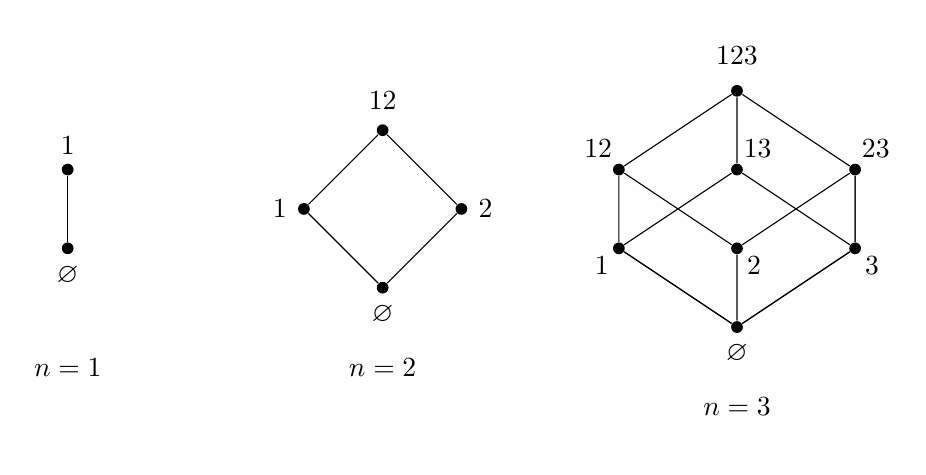
\begin{tikzpicture}[every node/.style={circle, fill, inner sep=1.5pt}]
    \begin{scope}[shift={(0,0.5)}]
    
    \node[label=above:{$1$}] (b) at (0,.5) {};
    \node[label=below:{$\emptyset$}] (a) at (0,-0.5) {};
    \node[below=0.5cm,fill=none] at (0,-1) {$n=1$};

    \draw (a) -- (b);
    \end{scope}

    \begin{scope}[shift={(3,.5)}] 
    \node[label=above:{$12$}] (12) at (1,1) {};
    \node[label=left:{$1$}] (1) at (0,0) {};
    \node[label=right:{$2$}] (2) at (2,0) {};
    \node[label=below:{$\emptyset$}] (0) at (1,-1) {};
    \node[below=0.5cm,fill=none] at (1,-1) {$n=2$};

    \draw (12) -- (1);
    \draw (12) -- (2);
    \draw (1) -- (0);
    \draw (2) -- (0);
    \end{scope}

    \begin{scope}[shift={(7,0)}] 
        \node[label=below left:{$1$}] (a1) at (0,0) {};
        \node[label=below right:{$2$}] (b1) at (1.5,0) {};
        \node[label=below right:{$3$}] (c1) at (3,0) {};
        \node[label=above left:{$12$}] (ab1) at (0,1) {};
        \node[label=above right:{$13$}] (ac1) at (1.5,1) {};
        \node[label=above right:{$23$}] (bc1) at (3,1) {};
        \node[label=above:{$123$}] (abc1) at (1.5,2) {};
        \node[label=below:{$\emptyset$}] (ee1) at (1.5,-1) {};
        \node[below=0.5cm,fill=none] at (1.5,-1) {$n=3$};

        \draw (abc1) -- (ab1) -- (a1) -- (ee1);
        \draw (abc1) -- (bc1) -- (c1) -- (ee1);
        \draw (abc1) -- (ac1) -- (a1) -- (ee1);
        \draw (ab1) -- (b1) -- (ee1);
        \draw (ac1) -- (c1);
        \draw (bc1) -- (b1);
        \draw (bc1) -- (c1) -- (ee1);
    \end{scope}
\end{tikzpicture}
\]
όπου δεν συμπεριλάβαμε τις αγκύλες για λόγους απλότητας (για παράδειγμα, με $12$ συμβολίζουμε το $\{1, 2\}$). Ένα ακόμη παράδειγμα μερικής διάταξης είναι ο σύνδεσμος ιδεωδών ενός δακτύλιου, που συναντήσαμε στην Ενότητα 1.

Ένα (μη κενό) υποσύνολο $\cC$ μιας μερικής διάταξης $(\pP,\leq)$ με την ιδιότητα $x \leq y$ ή $y \le x$ για κάθε $x, y \in \cC$ ονομάζεται \defn{αλυσίδα} (chain) του $\pP$. Για παράδειγμα, τα υποσύνολα $\{1\}$ και $\{1,2\}$ σχηματίζουν μια αλυσίδα του $2^{[3]}$, ενώ τα $\{1\}, \{2\}$ όχι. 

Τέλος, ένα στοιχείο $x \in \pP$ ονομάζεται \defn{άνω φράγμα} (upper bound) ενός υποσυνόλου $\qQ \subseteq \pP$ αν $y \le x$, για κάθε $y \in \qQ$. Για παράδειγμα, το στοιχείο $\{1,2\}$ είναι άνω φράγμα του $\{ \{1\}, \{1,2\} \}$ στο $2^{[3]}$.

\begin{zorn}
    Έστω $\pP$ μια (μη κενή) μερική διάταξη. Αν κάθε αλυσίδα του $\pP$ έχει άνω φράγμα, τότε το $\pP$ έχει μεγιστικό στοιχείο.
\end{zorn}

\begin{proof}[Απόδειξη του Λήμματος \ref{lem:maximal_ideal_existence}]
    Έστω $\pP$ το σύνολο όλων των γνήσιων ιδεωδών του $R$, ο σύνδεσμος ιδεωδών του $R$ χωρίς το ιδεώδες $R$. Τότε $\pP \neq \emptyset$, διότι $\{0_R\} \in \pP$. Έστω $\cC$ μια αλυσίδα του $\pP$. Από το Λήμμα του Zorn, αρκεί να δείξουμε ότι το $\cC$ έχει άνω φράγμα.

    Πράγματι, θεωρούμε το 
    \[
    J = \bigcup_{I \in \cC} I \ \in \ \pP,
    \]
    όμοια με την απόδειξη του Λήμματος 2.13. To $J$ είναι άνω φράγμα του $\cC$ (γιατί;) και η απόδειξη ολοκληρώνεται.
\end{proof}

\begin{thebibliography}{99}
    \bibitem{Alu09}
    P.~Aluffi,
    \textit{Algebra, Chapter 0},
    Grad. Stud. in Math. {\bf104},
    Amer. Math. Soc., Providence, RI, 2009.
    \bibitem{DF04}
    D. S. Dummit και R. M. Foote, 
    \textit{Abstract algebra},
    third edition, Wiley, 2004. 
\end{thebibliography}
\end{document}